\documentclass{beamer}
\usepackage{subfigure} 
\usepackage{amsopn}
%\usepackage{CJK}


\usetheme{Warsaw}
\title{Simultaneous Localization and Mapping With Dual Cameras}
\author{B97902018 Chun-Liang Li \and 
	B97902058 Po-Wei Wang}
\date{2012/06/26}


\begin{document}
	\begin{frame}
		\titlepage
	\end{frame}

	\begin{frame}{What is SLAM}
		\textbf{S}imultaneous \textbf{L}ocalization \textbf{A}nd \textbf{M}apping: 
		
		Build map within an unknown environment and keep track current localizations
		\begin{center}
			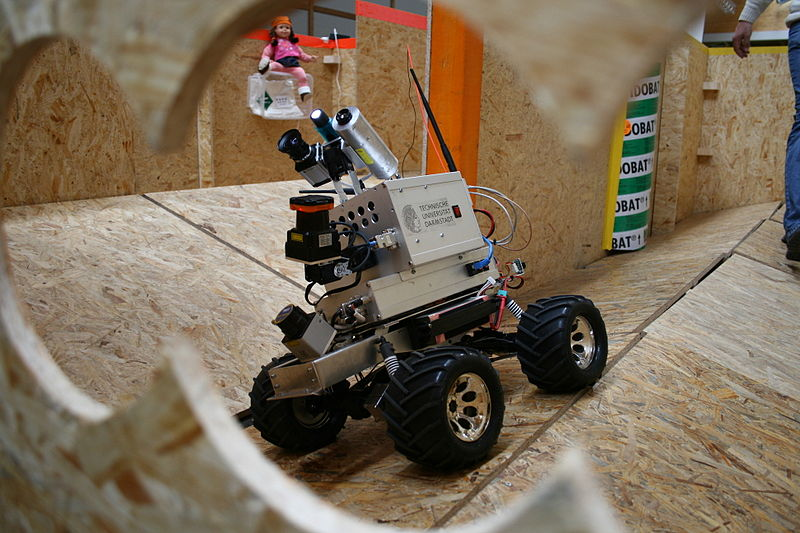
\includegraphics[width=0.5\textwidth]{./pics/robot.jpg} 
		\end{center}
	\end{frame}

	\begin{frame}{ Approaches (Devices) }
		How to observe environments ? Sensors, Cameras ... etc\\
		\begin{itemize}
			\item Sensor: more specific and accurate
			\item Camera: most intuitive and ubiquitous devices
		\end{itemize}
		\begin{center}
			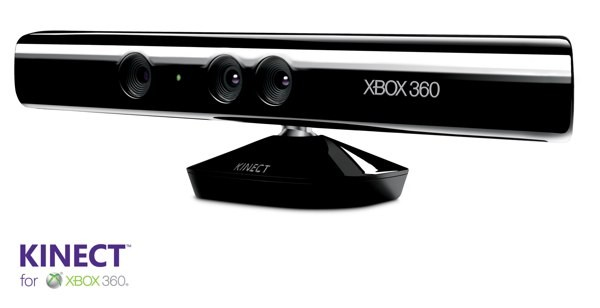
\includegraphics[width=0.5\textwidth]{./pics/sensor.jpg} 
		\end{center}
		\uncover<2->
		{
			
			A.J. Davison et al. MonoSLAM Real-Time Single Camera SLAM
		}
	\end{frame}
	
	\begin{frame}{Challenge}
		Single Camera: Hard to determine scene depth \\
		\uncover<2->
		{
			Dual Cameras: Easily to estimate positions
			\begin{center}
				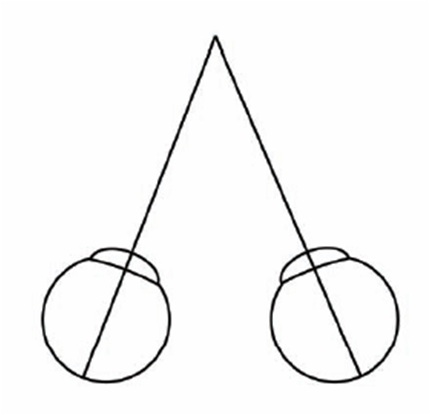
\includegraphics[width=0.5\textwidth]{./pics/dual.jpg} 
			\end{center}
			%put figures
		}
		\uncover<3->
		{
			Drawback: No Research work related to it ...
		}
	\end{frame}

	\begin{frame}{Hardware Hacks}
		Stereo systems are often bothered by time gaps between cameras.\\
		\uncover<2->
		{
			We choose PS3Eye and do some hardware hack (connect VSYN and FSIN)
			\begin{center}
				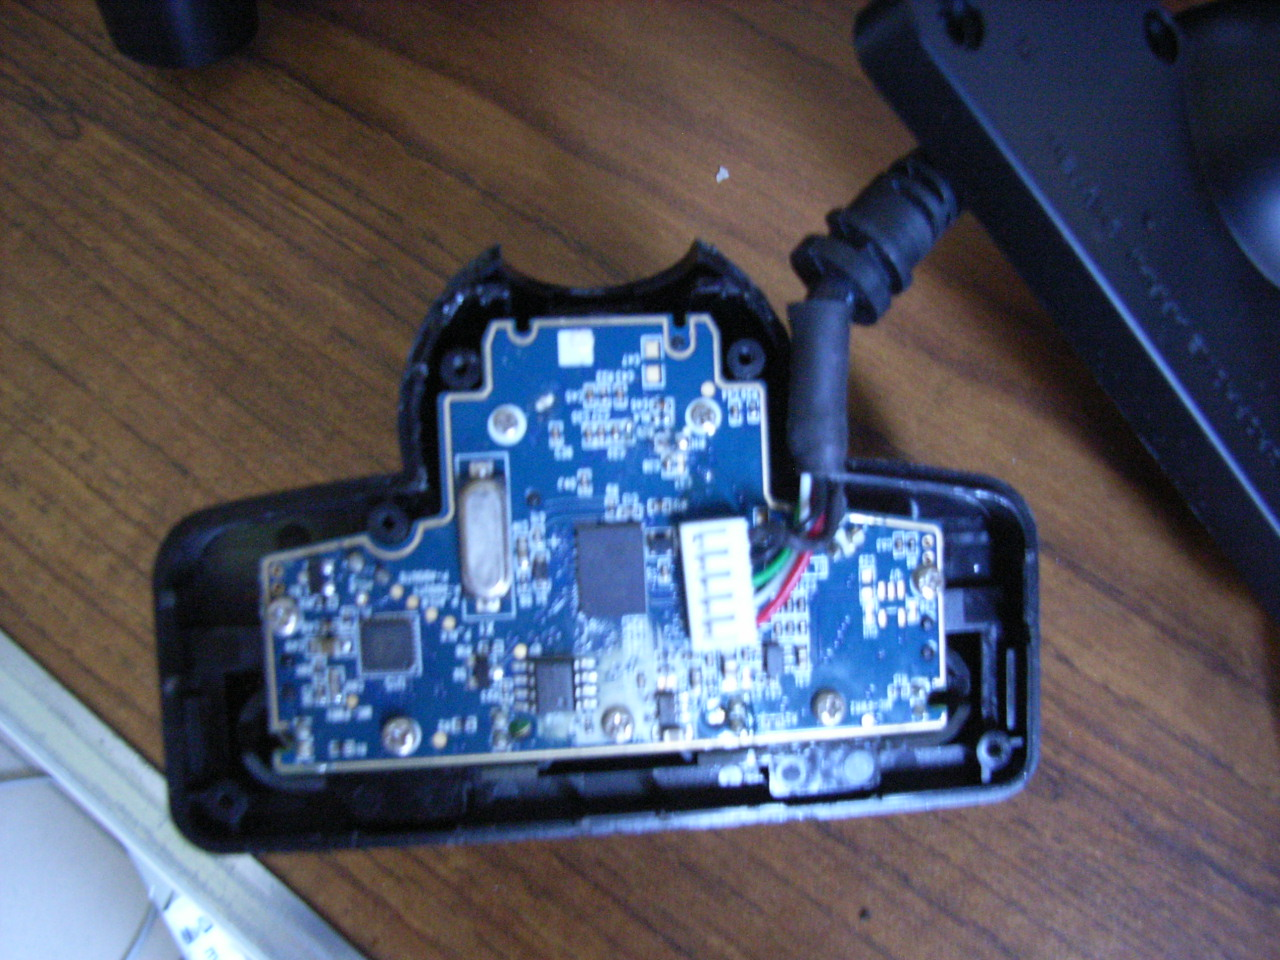
\includegraphics[width=0.5\textwidth]{./pics/mia_pcb.jpg} 
			\end{center}
			Result: 120fps 320x240 Synchornized Cameras.
		}
	\end{frame}

	\begin{frame}{The Third Eye}
		Bandwidth: 320x240 x 1.5(YUYV420p) x 120 x 2 = 26MBps\\
		USB2.0 theoretical = 35MBps\\
		If we want to record video at the same time..\\
		\uncover<2->
		{
			Logitech C920 H264 Hardware camera\\
			\begin{center}
				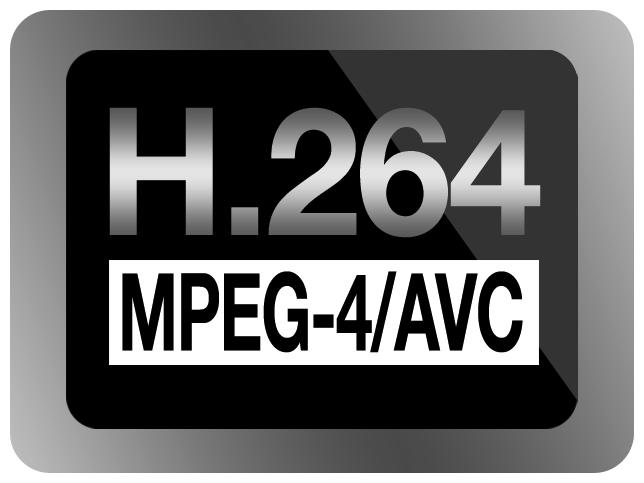
\includegraphics[width=0.5\textwidth]{./pics/h264-logo.png} 
			\end{center}
			Result: Highly compressed 1080p
		}
	\end{frame}

	\begin{frame}{Calibration}
		1-1. Stereo Calibration\\
		1-2. Test Reprojection Error\\
		2-1. Determin the extrinsics of HD Cam\\
		2-2. Project the 3D from Stereo to HD Cam
		\begin{center}
			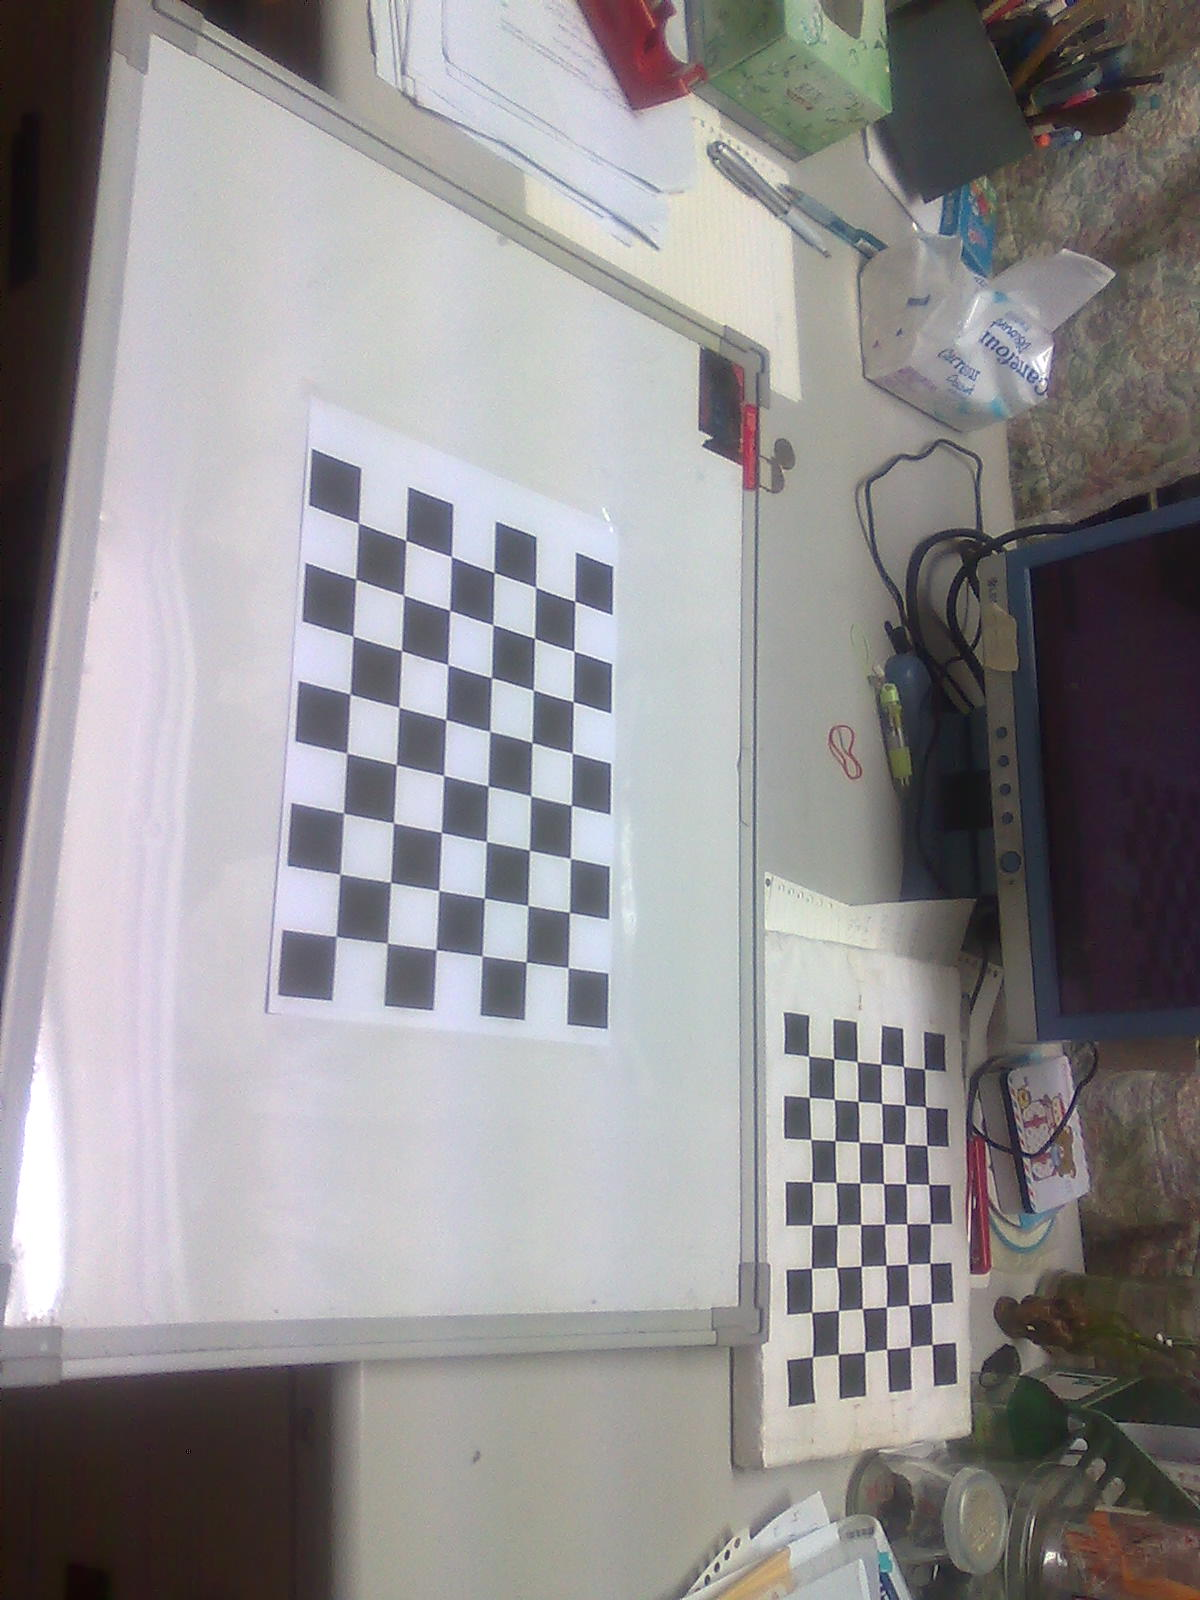
\includegraphics[width=0.3\textwidth]{./pics/chessboard.jpg} 
		\end{center}
	\end{frame}

	\begin{frame}{From Image to Matches}
		\begin{center}
			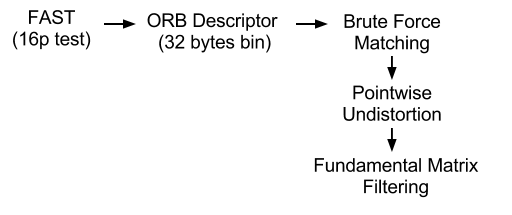
\includegraphics[width=0.8\textwidth]{./pics/feats.png} 
		\end{center}
		
		\begin{center}
			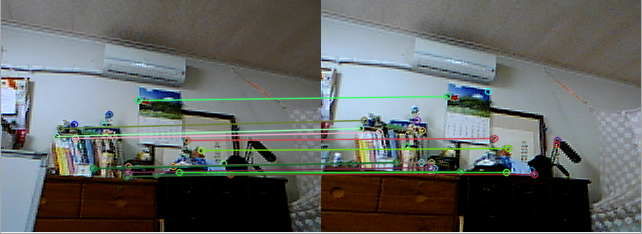
\includegraphics[width=0.8\textwidth]{./pics/match.png} 
		\end{center}
	\end{frame}

	\begin{frame}{Extended Kalman Filter Algorithm}
		One of the most common algorithm in SLAM.\\
		%put prediction and measurement figure
		\uncover<2->
		{
			\begin{center}
				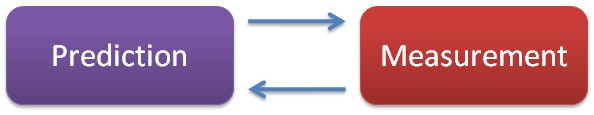
\includegraphics[width=0.5\textwidth]{./pics/ekf.jpg} 
			\end{center}
			\begin{itemize}
				\item Prediction: predict current camera positions \alert{$f(x)$}
				\item Measurement: estimate the position of object $y$, \alert{$h(x,y)$}, in local frame and update map based on the residual
			\end{itemize}
		}
		\uncover<3->
		{
			\[
			\mathbf{x} = \left( 
			\begin{array}{c} 
				\mathbf{r}\\
				\mathbf{q}\\
				\mathbf{v}\\
				\mathbf{\omega}\\
			\end{array}
			\right),  
			f\left( 
			\begin{array}{c} 
				\mathbf{r}\\
				\mathbf{q}\\
				\mathbf{v}\\
				\mathbf{\omega}\\
				\Delta t
			\end{array} 
			\right) = 
			\left( 
			\begin{array}{c}
				\mathbf{r} + (\mathbf{v}+\mathbf{V})\Delta t\\
				\mathbf{q}((\mathbf{\omega}+\mathbf{\Omega})\Delta t) \times \mathbf{q}\\
				\mathbf{v} + \mathbf{V}\\
				\mathbf{\omega} 
			\end{array} 
			\right)
			\] \\

			\[ h(x,y) = R(\mathbf{q})^{-1}( \mathbf{y}-\mathbf{r} ) \]
		}
	\end{frame}

	\begin{frame}{Extended Kalman Filter Algorithm}
		Full Algorithm: \\
		\[ A \equiv \frac{ \partial f(\mathbf{x}) }{ \partial \mathbf{x} } \]
		\[ H \equiv \frac{ \partial h(\mathbf{x},\mathbf{y}) }{ \partial \mathbf{x} } \]
		prediction:\\
		\[\mathbf{x} = f(\mathbf{x})\]
		\[\Sigma = A\Sigma A^{T} + Q\]
		measurement:\\
		\[K = \Sigma H^{T}(H\Sigma H^{T}+R)^{-1}\]
		\[\mathbf{x} = \mathbf{x}+K(z-h(\mathbf{x},\mathbf{y}))\]
		\[\Sigma = (I-KH)\Sigma\]


	\end{frame}
\end{document}
